%\documentclass[12pt]{article}
%\usepackage[a4paper, margin=1in]{geometry} 
%\usepackage{graphicx} 
%\usepackage{hyperref}
%\usepackage{float}
%\usepackage{multicol}
%\usepackage{multirow}
%\usepackage[font=small, labelfont=bf]{caption}
%
%\begin{document}

%
% Biological databases
%
 \subsection{Biological databases}
Biological databases contain biological information, mainly collected from molecular biology experiments, life science literature, and bioinformatics analyses.

%
% Categories of databases
%
\subsubsection*{Categories of databases} 
Annual \href{http://nar.oxfordjournals.org}{Nucleic Acids Research} database issue includes the following database categories.

\begin{itemize}
\item Nucleotide Sequence Databases
\item RNA sequence databases
\item Protein sequence databases
\item Structure Databases
\item Proteomics Resources
\item Human and other Vertebrate Genomes
\item Genomics Databases (non-vertebrate)
\item Plant databases
\item Human Genes and Diseases
\item Metabolic and Signaling Pathways
\item Immunological databases
\item ...
\end{itemize}

%
% GenBank
%
\subsubsection*{GenBank} 
\begin{itemize}
\item A comprehensive database of publicly available nucleotide sequences
\item Produced and maintained by NCBI (National Center for Biotechnology Information, URL: \href{http://www.ncbi.nlm.nih.gov}{http://www.ncbi.nlm.nih.gov})
\end{itemize}

\begin{figure}[H]
  \centering
      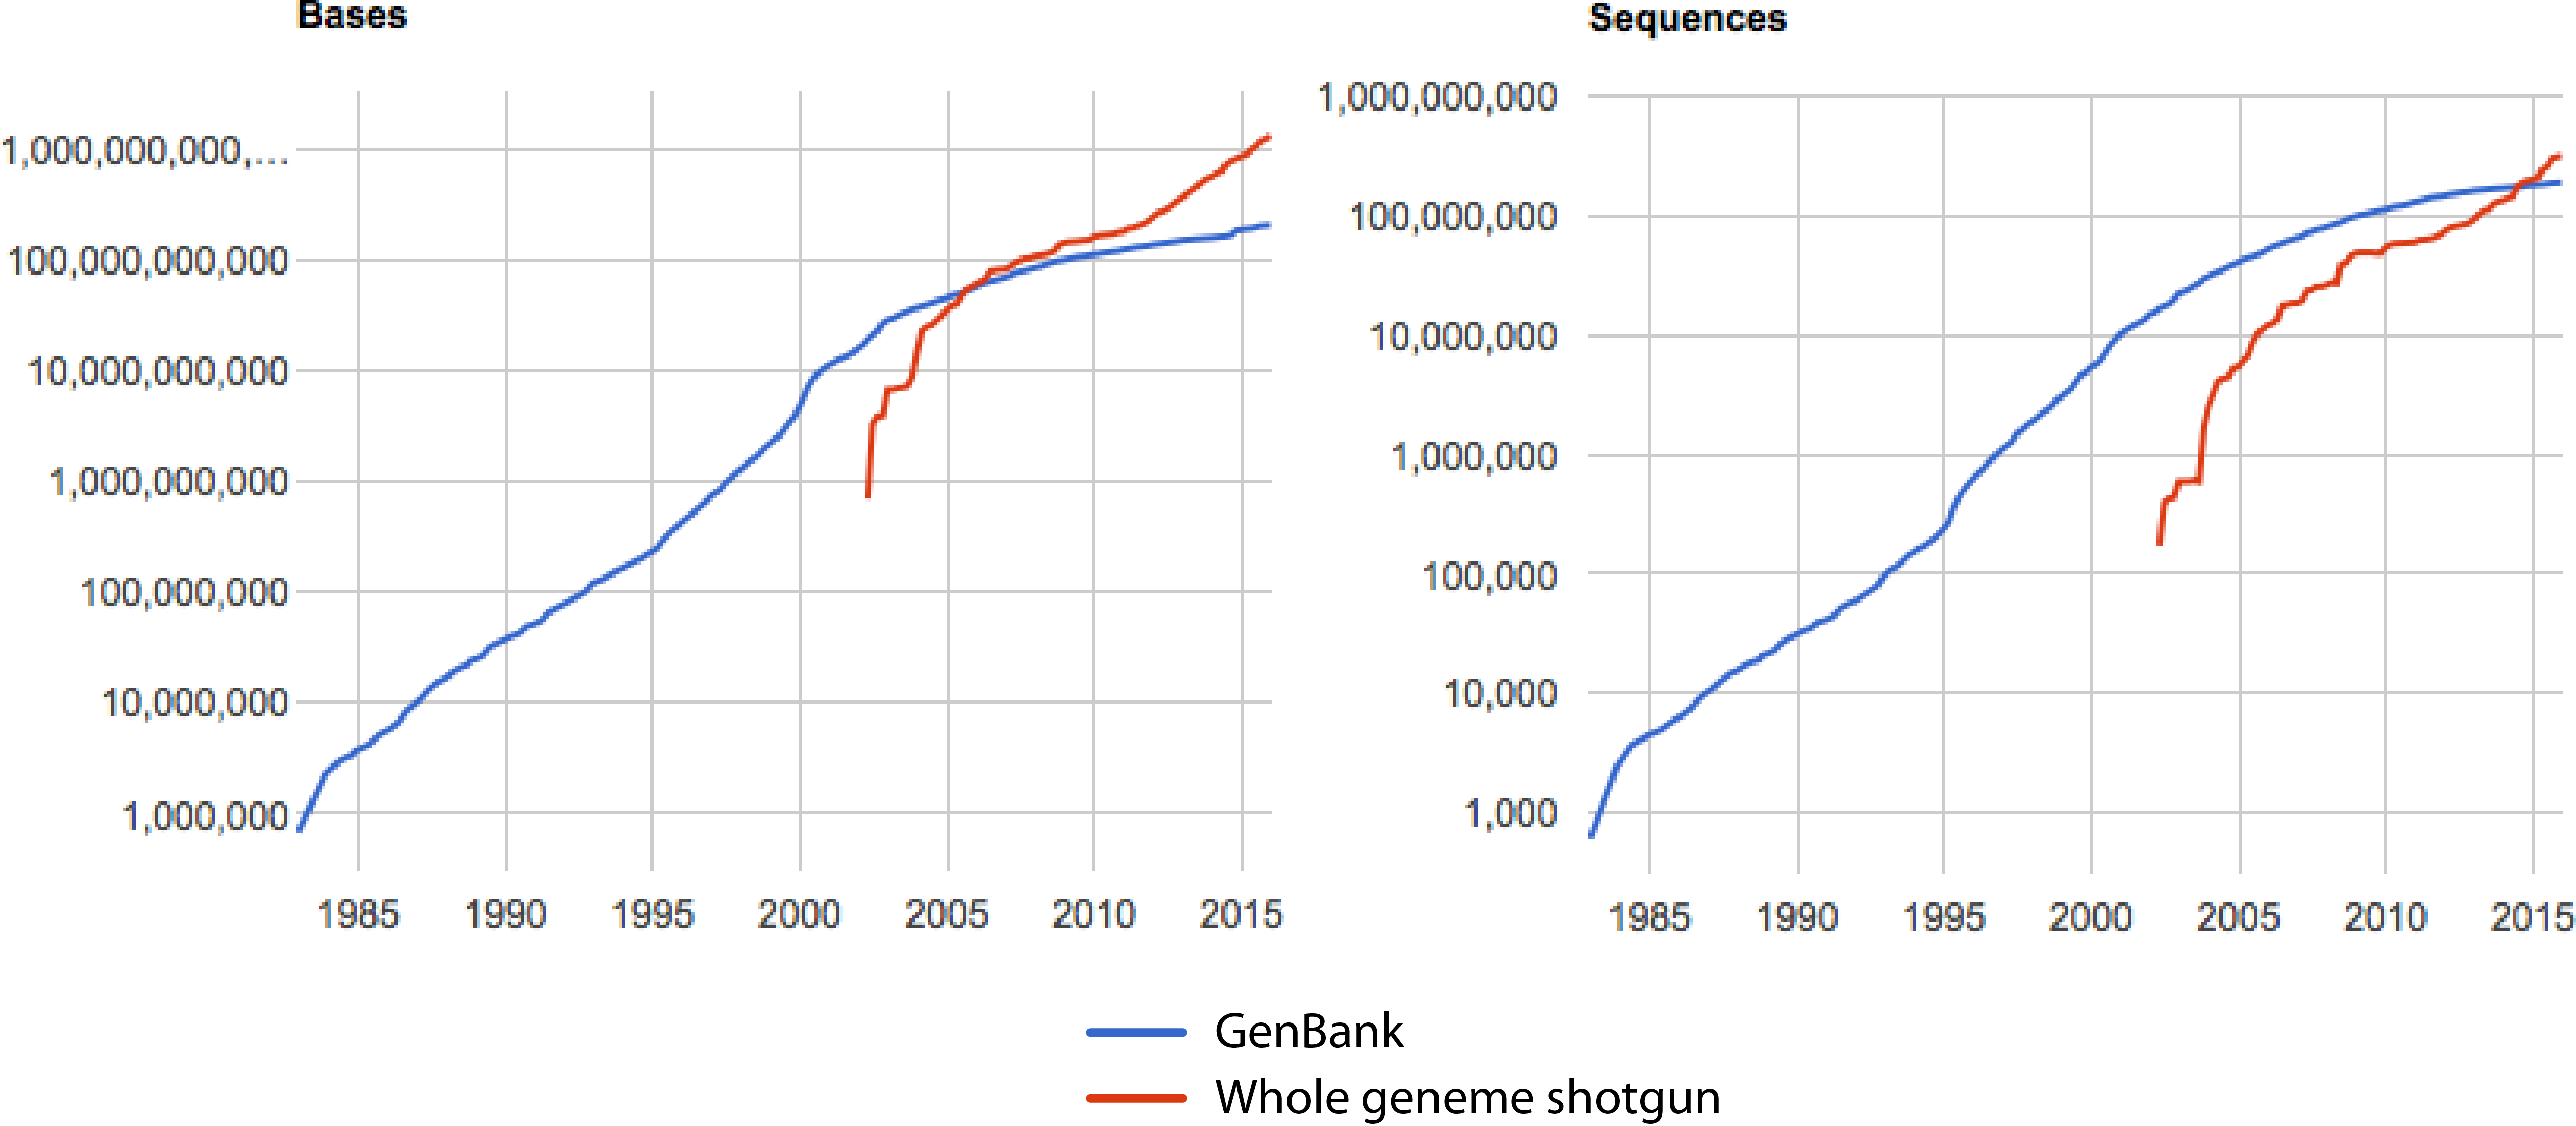
\includegraphics[width=0.6 \textwidth]{fig05/genebank_stat.png}
  \caption{Growth of GenBank and WGS (source: \href{http://www.ncbi.nlm.nih.gov/genbank/statistics}{NCBI})}
\end{figure}

%
% UniProt
%
\subsubsection*{UniProt} 
\begin{itemize}
\item A central repository of protein data from Swiss-Prot, TrEMBL, and PIR-PSD databases
\item Maintained by the UniProt consortium
\end{itemize}

%
% Sequence data 
%
\subsubsection*{Sequence data} 
\begin{itemize}
\item Identifier
\item Sequence
\end{itemize}

\noindent
\textbf{Data format of sequence data} \\
FASTA is the most popular format for sequence data.
\begin{figure}[H]
  \centering
      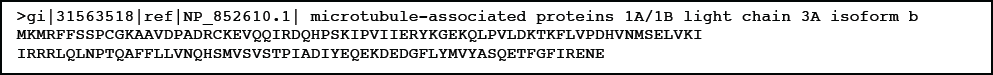
\includegraphics[width=\textwidth]{fig05/fasta.png}
\end{figure}

%
% Annotation data
%
\subsubsection*{Annotation data} 
Sequences databases usually contain annotations in addition to sequences. 

\begin{itemize}
\item Notes and descriptions of important regions and components
\item Meta data
\end{itemize}

\noindent
\textbf{Data format of annotation data} \\
Annotation data can be downloaded in many different formats. GFF is one of the popular file formats for storing genomic features.
\begin{figure}[H]
  \centering
      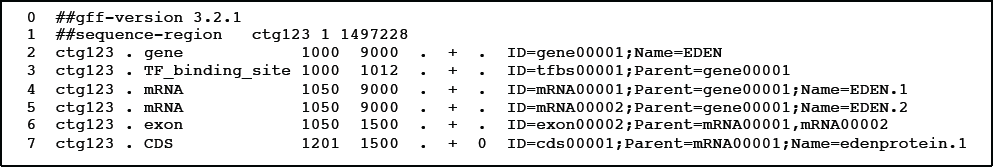
\includegraphics[width=\textwidth]{fig05/gff3.png}
\end{figure}

%
% Tools
%
\subsubsection*{Tools}
Many database tools are available for various purposes.
 
\noindent
\textbf{Search tools for sequence databases}
\begin{itemize}
\item BLAST at NCBI (\href{http://blast.ncbi.nlm.nih.gov/Blast.cgi}{http://blast.ncbi.nlm.nih.gov/Blast.cgi})
\item BLAT/BLAST at Ensembl (\href{http://www.ensembl.org/Multi/Tools/Blast}{http://www.ensembl.org/Multi/Tools/Blast})
\end{itemize}

\noindent
\textbf{Data browsing tools of annotation and sequence data}
\begin{itemize}
\item UCSC Genome Browser (\href{https://genome.ucsc.edu}{https://genome.ucsc.edu})
\item Ensemble Genome Browser (\href{http://www.ensembl.org}{http://www.ensembl.org})
\end{itemize}

\noindent
\textbf{Data download tools for annotation and sequence data}
\begin{itemize}
\item UCSC Table Browser (\href{http://genome.ucsc.edu/cgi-bin/hgTables}{http://genome.ucsc.edu/cgi-bin/hgTables})
\item Ensemble BioMart (\href{http://www.ensembl.org/biomart}{http://www.ensembl.org/biomart})
\end{itemize}

\noindent
\textbf{Tools for protein data}
\begin{itemize}
\item UniProt (\href{https://www.uniprot.org}{https://www.uniprot.org})
\end{itemize}

\bigskip 

%\end{document}
